\documentclass{article}
\usepackage[a4paper, margin=3cm]{geometry}
\usepackage[utf8]{inputenc}
\usepackage{hyperref}
\usepackage{graphicx}
\usepackage{listings}

\title{mlcommons tiny (v0.5) performance benchmark on NVIDIA Jetson Nano Developer Kit, keyword spotting case}
\author{Daniel Morandini, dmorandini@unibz.it (12286)}
\date{August 2021}

\begin{document}
\maketitle

\section{Introduction}
MLCommons\footnote{\url{https://mlcommons.org/en}} is working on a variety of benchmarks aimed towards classifying the performance and energy consumption, and hence the suitability, of hardware platforms when used for machine learning inferences. The tiny\footnote{\url{https://mlcommons.org/en/inference-tiny-05}} benchmark is reserved for microcontrollers and devices that may be deployed for "Edge" computing, i.e. when computationally expensive ML\footnote{Machine Learning} operations are performed near the data source "in the field". This is a companion technique of Cloud computing, where raw data is sent to a data center for processing. Devices on the field usually have limited computational power, memory and energy available compared to servers in a data center; for this reason finding the most suitable device for deploying, for example, an image processing application backed by a CNN\footnote{Convolutionary Neural Network} engine (which is notoriously energy, memory and hence power hungry) that draws its energy from a relatively small rechargeable battery is far from being trivial.

This report evaluates the experience of porting such benchmark on the NVIDIA Jetson Nano Developer Kit\footnote{\url{https://www.nvidia.com/it-it/autonomous-machines/embedded-systems/jetson-nano}}. The v0.5 of the framework comprises four different tests, being \textbf{Keyword Spotting}, \textbf{Visual Wake Words}, \textbf{Image classification}, \textbf{Anomaly Detection}. This project focused its efforts on the Keyword Spotting case only, which will be analysed in detail in section \ref{kws}.

\section{Hardware}\label{hw}
This section will provide an overview of the hardware capabilities of this project's target machine, i.e. the Nvidia Jetson Nano Developer Kit or Jetson for brevity, which are relevant for the purposes of the benchmark. For the full story, read the datasheet\footnote{\url{https://developer.nvidia.com/embedded/dlc/jetson-nano-system-module-datasheet}}.

The machine is composed by the "peripheral" PCB, comprising, among other components, a Gigabit Ethernet connector, USB-3/2/mini ports, power jack, GPIO pins and the proper Jetson SoM connected with the rest of the board through a PCIe interface.
\begin{figure}[h]
    \centering
    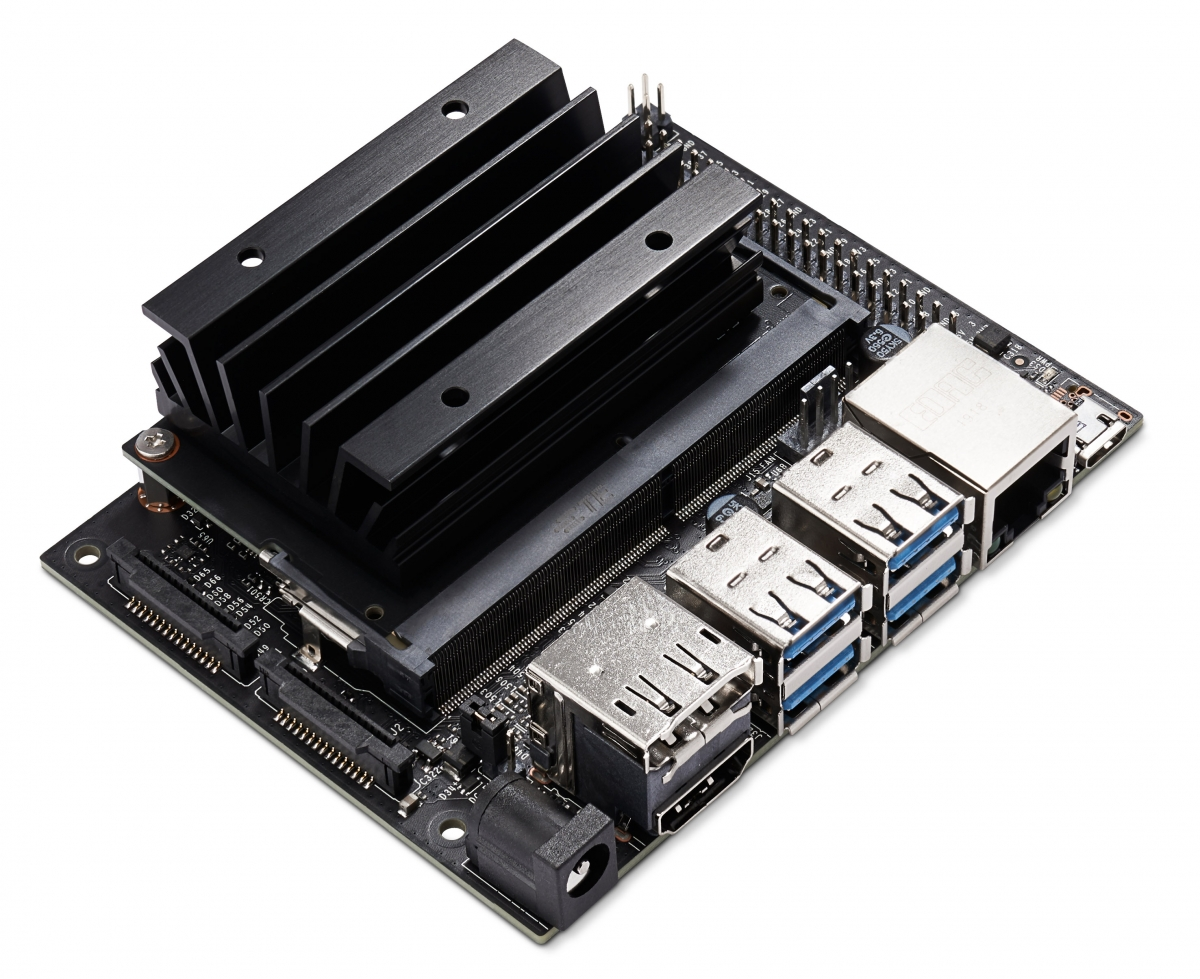
\includegraphics[width=.5\textwidth]{assets/JetsonNano-DevKit_Front-Top_Right_trimmed.jpg}
    \caption{NVIDIA Jetson Nano Developer Kit}
    \label{fig:jetsonnano}
\end{figure}
Let us turn our attention to the SoM only; removing the heatsink we find an NVIDIA Tegra X1 series SoC featuring an ARM Cortex-A57 (quad-core, 64bit) Processor with NEON Technology. The memory hierarchy of the CPU is composed by 48KB of L1 instruction cache (per core), 32KB of L1 data cache (per core) and a global L2 unified cache of 2MB. The maximum reported operating frequency is 1.43GHz.

The chip is also equipped with a 128-core NVIDIA Maxwell GPU performing up to 512 GFLOPS (FP16) and a maximum operating frequency of 921MHz, software tunable (as the CPU frequency is) through the "Tegra Power and Thermal Management Software".

The Linux distribution provided by sdkmanager includes a tool called jetson\_clocks that can be used to obtain actual clock frequencies. Listing \ref{lst:clk} shows the obtained results in Hz (eliding less relevant content for brevity), i.e. \textbf{1.47MHz} on the CPU cores and \textbf{921MHz} on the GPU.

\begin{lstlisting}
cpu0: MinFreq=1479000 MaxFreq=1479000 CurrentFreq=1479000
cpu1: MinFreq=1479000 MaxFreq=1479000 CurrentFreq=1479000
cpu2: MinFreq=1479000 MaxFreq=1479000 CurrentFreq=1479000
cpu3: MinFreq=1479000 MaxFreq=1479000 CurrentFreq=1479000
GPU MinFreq=921600000 MaxFreq=921600000 CurrentFreq=921600000
EMC MinFreq=204000000 MaxFreq=1600000000 CurrentFreq=1600000000
\end{lstlisting}\label{lst:clk}

The Jetson integrates a 4GB of LPDDR4 over a four-channel 16-bit interface. Memory frequency options (managed by the memory controller) are 204MHz and 1.6GHz; as shown in listing \ref{lst:clk}, the selected memory controller frequency is \textbf{1.6GHz}. the theoretical peak memory bandwidth is 25.6GB/s. A memory bandwidth test has been conducted between CPU-GPU (here referred to as host and device respectively), GPU-CPU and GPU-GPU. Results are reported in listing \ref{lst:membw} and show that the "theoretical speed" is far from being hit. Tests performed with different transfer sizes (notably with 12000000 Bytes or 12MB) reached but never exceeded speeds of 10.6GB/s between CPU-GPU and vice-versa.
\begin{lstlisting}[caption=CUDA Memory Bandwidth Test within NVIDIA Tegra X1]
=================================================================
Transfer Size: 32MB (PINNED)

Host to Device:    5.6GB/s
Device to Host:    10.5GB/s
Device to Device:  16.7GB/s
=================================================================
\end{lstlisting}\label{lst:membw}

\section{Software Stack(s)}\label{sws}
NVIDIA provides a tool called sdkmanager v1.6\footnote{version used is 1.6, https://developer.nvidia.com/nvidia-sdk-manager} that can be used to flash the SD card inserted in the Jetson module while the board is in \textit{recovery mode}\footnote{triggered by bridging the FC REC pin on the J50 connector to GND on startup}. The tool is used in an iterative fashion to find out the desired command line flags. Follows the full sdkmanager command.
\begin{lstlisting}[language=bash]
% sdkmanager --cli install  --logintype devzone --product Jetson \
--targetos Linux --version 4.6 --target JETSON_NANO_TARGETS --flash all
\end{lstlisting}
The tool takes care of populating the SD card with the necessary partitions for bootstrapping Ubuntu 18.04\footnote{Ubuntu 18.04.5 LTS (GNU/Linux 4.9.253-tegra aarch64)} with access to all peripherals (the proper Board Support Package is handed to Linux \footnote{Linux jetson 4.9.253-tegra SMP PREEMPT Mon Jul 26 12:13:06 PDT 2021 aarch64 aarch64 aarch64 GNU/Linux}), as well as the drivers required to work with the GPU. Futhermore, NVIDIA provides libraries build on top of the CUDA\footnote{\url{https://developer.nvidia.com/cuda-zone}} runtime tailored for ML applications, such as cuDNN\footnote{\url{https://developer.nvidia.com/cudnn}}, which can be installed with the sdkmanager as well, and they were.
The tiny benchmark v0.5 is divided into an open and a closed division. The former allows for whatever implementation, and in particular, whatever ML model implementers want to deploy to solve the problem at the cost of loosing the direct benchmark comparison across platforms. The latter, the one chosen in this project, does the opposite: implementers have to stick with the official ML learning model provided by MLCommons, building their solution on top of it, even though other approaches would be better suited for the job.
The model provided for the Keyword Spotting case is a protocol buffer\footnote{\url{https://developers.google.com/protocol-buffers}} encoded Tensorflow\footnote{\url{https://www.tensorflow.org}} graph comprising a four stage DS-CNN, built using the Keras framework\footnote{\url{https://keras.io}}. Model's structure and details will be covered in section \ref{perf}.

To be able to directly use the provided model, the Tensorflow's C library (with CUDA support) has been installed, together with its C API headers.

The benchmark is driven by the EMBC's eneryrunner tool\footnote{\url{https://github.com/eembc/energyrunner}} which has to be installed on a supported, extra machine. Details on the setup will be provided in section \ref{stp}.

The whole project is publicly available on Github at \url{https://github.com/jecoz/mlperf-jetson}.

\section{Setup}\label{stp}
Jetson needs to be connected to a power outlet through its J25 barrel jack connector. The J48 bridge has to be closed otherwise power will be expected from the micro-USB cable, which purpose instead is serial communication between the driver machine and the target. Once the two machines are connected, the Jetson is instructed to start the benchmark runner, which will wait for commands on the serial device. An example session on the Jetson follows.
\begin{lstlisting}[language=bash]
dan@jetson:~/p/mlperf-jetson/src$ make
cc -std=c11 -I. -g -Wno-discarded-qualifiers -c runner.c -o runner.o
cc -std=c11 -I. -g -Wno-discarded-qualifiers -c tf.c -o tf.o
cc -std=c11 -I. -g -Wno-discarded-qualifiers -c stdlib.c -o stdlib.o
cc -std=c11 -I. -g -Wno-discarded-qualifiers -c th.c -o th.o
g++ -o /home/dan/p/mlperf-jetson/src/bin/runner api/internally_implemented.o \
	runner.o tf.o stdlib.o th.o -lm -ltensorflow -g
cc -std=c11 -I. -g -Wno-discarded-qualifiers -c infer.c -o infer.o
cc -o /home/dan/p/mlperf-jetson/src/bin/infer infer.o tf.o \     
    stdlib.o -lm -ltensorflow -g

dan@jetson:~/p/mlperf-jetson/src$ source pre.sh
dan@jetson:~/p/mlperf-jetson/src$ bin/runner
line=/dev/ttyGS0 model_dir=kws_ref_model tf=2.3.1
initializing serial port...done
m-timestamp-mode-performance
m-lap-us-170647
initializing tensorflow...done
m-init-done
m-ready
\end{lstlisting}

On the driver machine, in this case an Apple device\footnote{MacBook Pro (Retina, 13-inch, Mid 2014) running macOS BigSur 11.5.2}, the benchmark tool is started. It will first scan serial devices issuing a "name" command. If a suitable response is received, the device is recognised and listed. It is up to the user then to configure the desired benchmark, initialize the device and issue inferences. Figure \ref{fig:embc} shows the benchmark after device initialization.
\begin{figure}[h]
    \centering
    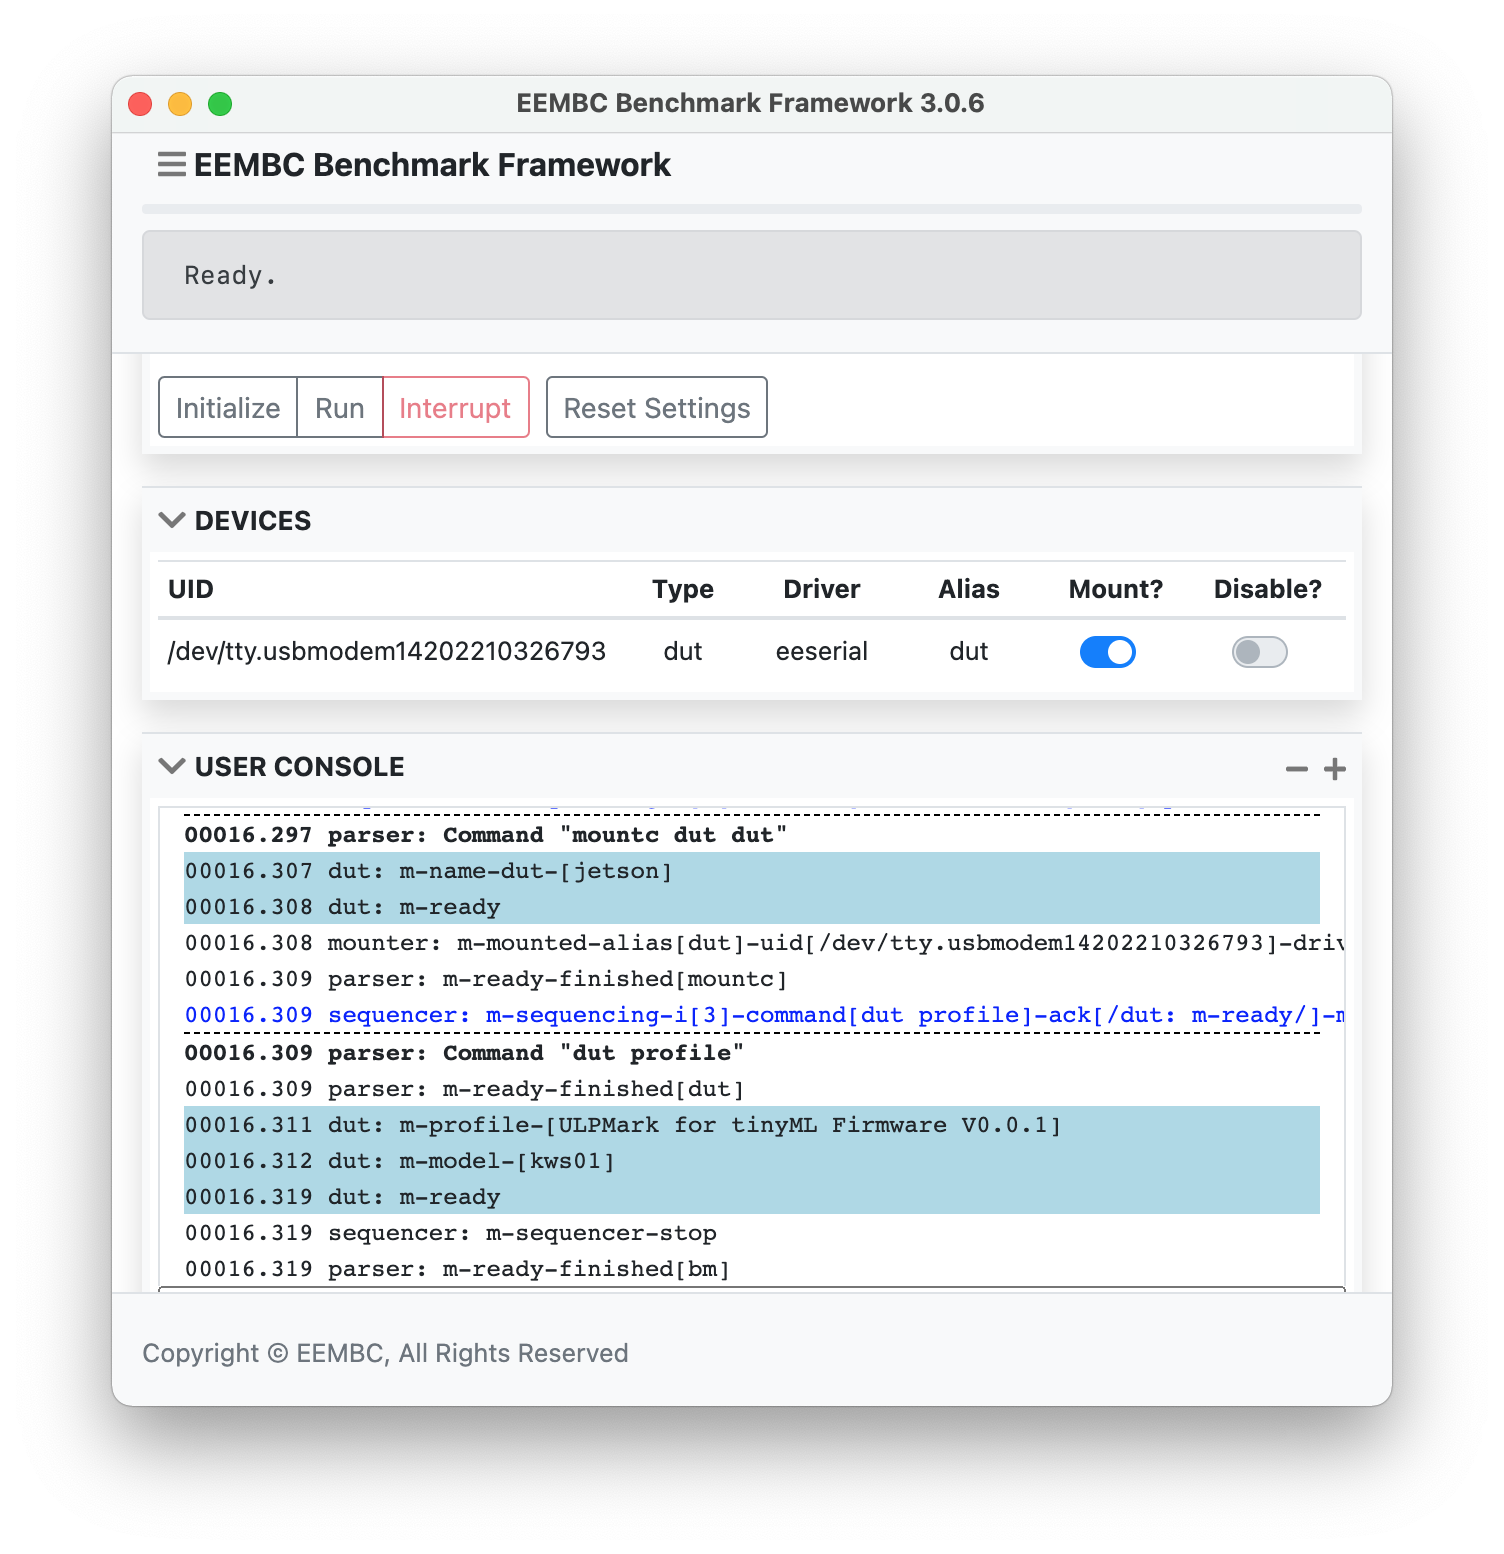
\includegraphics[width=.8\textwidth]{assets/Screenshot 2021-08-25 at 17.34.23.png}
    \caption{EMBC Host Benchmark Framework appearance after target device initialization}
    \label{fig:embc}
\end{figure}

\section{The Keyword Spotting Benchmark}\label{kws}
This benchmark aims at measuring solutions that spot specific words or brief phrases within an audio stream consuming as less power as possible. A common usecase is "wakeword" detection, used when a device has to wait for a specific user command, in this case vocal, before triggering intensive operations (e.g. Apple's "Hey Siri"). The detector continuously processes an audio stream monitoring the presence of such words, and if it were not power efficient it would not be deployed at all as listening alone would consume all device's power without achieving any goal.

The dataset is used by the benchmark is the curated Speech Commands v2 dataset, a collection of 105,829 utterances collected from 2,618 speakers with a variety of accents \footnote{P. Warden. Speech commands: A dataset for limited-vocabulary speech recognition. arXiv preprint arXiv:1804.03209, 2018.}.

Twelve command categories are used (the dataset provides more), which are "down", "go", "left", "no", "off", "on", "right", "stop", "up", "yes", "silence" and "unknown". The device-under-test is required to infer the audio category provided a MFSC\footnote{Mel-Frequency Spectral Coefficients} array of 490B, each point being a signed INT8. For a submission to be accepted, an accuracy of more than 90\% has to be achieved\footnote{\url{https://arxiv.org/pdf/2106.07597.pdf}}.

\section{Results}\label{got}
In this section, inference results will be accessed as provided by the framework without making any consideration on whether the performance of the system meets our expectations, i.e. whether it is "good" or "bad" on our hardware. That topic will be covered in section \ref{perf}.

Follows the output of both performance benchmarks provided by the framework.

\begin{lstlisting}[caption=Median Performance Result]
Performance results for window 2:
  # Inferences :         2400
  Runtime      :       10.309 sec.
  Throughput   :      232.803 inf./sec.
Runtime requirements have been met.
Performance results for window 4:
  # Inferences :         2400
  Runtime      :       10.296 sec.
  Throughput   :      233.105 inf./sec.
Runtime requirements have been met.
Performance results for window 6:
  # Inferences :         2400
  Runtime      :       10.362 sec.
  Throughput   :      231.609 inf./sec.
Runtime requirements have been met.
Performance results for window 8:
  # Inferences :         2400
  Runtime      :       10.382 sec.
  Throughput   :      231.177 inf./sec.
Runtime requirements have been met.
Performance results for window 10:
  # Inferences :         2400
  Runtime      :       10.333 sec.
  Throughput   :      232.260 inf./sec.
Runtime requirements have been met.
---------------------------------------------------------
Median throughput is 232.260 inf./sec.
---------------------------------------------------------
\end{lstlisting}\label{lst:perf}
Compared to the submitted reference results\footnote{\url{https://mlcommons.org/en/inference-tiny-05}}, which are compared in \textbf{inference delay in ms}\footnote{\(d = (1 / ips) * 1000\), where \(d\) is inference delay and \(ips\) inferences per second}, this implementation ranks 3/6 with its \textbf{4.3ms}, behind two Raspeberry Pi 4\footnote{\url{https://www.raspberrypi.org/products/raspberry-pi-4-model-b/}} using the LEIP Framework\footnote{\url{https://arxiv.org/abs/2103.06231}} that scored \textbf{0.39ms} and \textbf{0.42ms} respectively, which for the former result, is a \textbf{10.2x} speedup.

\begin{lstlisting}[caption=Accuracy Benchmark Result]
Top-1: 8.6%
AUC: 0.50
\end{lstlisting}\label{lst:acc}
Results displayed in listing \ref{lst:acc} show the flaw of this project: accuracy requirements have not been met yet. Our DS-CNN associates every sample (with varying accuracy) with the "unknown" category. The cause has not been identified at the time of writing, but what has been verified is that the model's graph is correctly loaded by the Tensorflow library, hence chances are high that the weights and/or biases are not being included correctly. The training procedure instead, which verifies the produced graph before storing it, reports the expected model accuracy.

\section{Performance Analysis}\label{perf}
This section's goal is finding performance inefficiencies in the proposed implementation. This analysis is inspired by the formal method presented by Marco Iodice at the Embedded Vision Summit, 2019\footnote{\url{https://www.edge-ai-vision.com/2019/07/performance-analysis-for-optimizing-embedded-deep-learning-inference-software-a-presentation-from-arm}}.

Let us first begin by collecting the \textbf{computational cost} and \textbf{memory footprint} of the model's graph, which shape is described in listing \ref{lst:model}.
\begin{lstlisting}
_________________________________________________________________
Layer (type)                 Output Shape              Param #   
=================================================================
input_1                      [(None, 49, 10, 1)]       0         
conv2d                       (None, 25, 5, 64)         2624      
batch_normalization          (None, 25, 5, 64)         256       
activation                   (None, 25, 5, 64)         0         
dropout                      (None, 25, 5, 64)         0         
depthwise_conv2d             (None, 25, 5, 64)         640       
batch_normalization_1        (None, 25, 5, 64)         256       
activation_1                 (None, 25, 5, 64)         0         
conv2d_1                     (None, 25, 5, 64)         4160      
batch_normalization_2        (None, 25, 5, 64)         256       
activation_2                 (None, 25, 5, 64)         0         
depthwise_conv2d_1           (None, 25, 5, 64)         640       
batch_normalization_3        (None, 25, 5, 64)         256       
activation_3                 (None, 25, 5, 64)         0         
conv2d_2                     (None, 25, 5, 64)         4160      
batch_normalization_4        (None, 25, 5, 64)         256       
activation_4                 (None, 25, 5, 64)         0         
depthwise_conv2d_2           (None, 25, 5, 64)         640       
batch_normalization_5        (None, 25, 5, 64)         256       
activation_5                 (None, 25, 5, 64)         0         
conv2d_3                     (None, 25, 5, 64)         4160      
batch_normalization_6        (None, 25, 5, 64)         256       
activation_6                 (None, 25, 5, 64)         0         
depthwise_conv2d_3           (None, 25, 5, 64)         640       
batch_normalization_7        (None, 25, 5, 64)         256       
activation_7                 (None, 25, 5, 64)         0         
conv2d_4                     (None, 25, 5, 64)         4160      
batch_normalization_8        (None, 25, 5, 64)         256       
activation_8                 (None, 25, 5, 64)         0         
dropout_1                    (None, 25, 5, 64)         0         
average_pooling2d            (None, 1, 1, 64)          0         
flatten                      (None, 64)                0         
dense                        (None, 12)                780       
=================================================================
\end{lstlisting}\label{lst:model}
The computational cost can be obtained summing the operations required by each layer. Some layers, such as dropout, flatten, batch\_normalization+activation are computationally inexpensive during inference, while others, such as convolutions and fully connected layers (dense), are. Convolution cost can be computed as \[MACC_{conv} = K_w * K_h * C_{in} * H_{out} * W_{out} * C_{out}\] where \(K_*\) refers to Kernel while \(C_*\), \(W_*\) and \(H_*\) the tensor's Channel, Width and Height properties respectively. A Depthwise Separable convolution is instead computed by two distinct operations, the former being the "depthwise" part that is basically equivalent to a normal convolution but does not combine input layers (input and output channels are the same), hence the formula becomes \[MACC_{dwconv} = K_w * K_h * C * H_{out} * W_{out}\]
The second portion is a pointwise (\(K*K=1)\) convolution, hence \[MACC_{pwconv} = C_{in} * H_{out} * W_{out} * C_{out}\]
The last computationally intensive layer is the dense one, which MACCs can be computed multiplying input and output channel vectors.
In terms of FLOPs (FLoating point OPerations, count only), given two vectors of size \(n\) a dot product performs \(2n - 1\) FLOPS since there are \(n\) multiplications and \(n - 1\) additions. Hence FLOPs can be estimated as being \(FLOP ~= 2*MACC\)\footnote{\url{https://machinethink.net/blog/how-fast-is-my-model/}}.
Combining the hardware specs depicted in section \ref{hw}, in particular recalling that the peak FLOPS (FLoating point OPerations per Second) reported by NVIDIA is 512 GFLOPS (FP16!), we can obtain the theoretical execution time by dividing the estimated required operations by the operations per second that our machine can execute, obtaining \textbf{6.5µs}\footnote{\(3.329MFLOPs / 512000MFLOPS = 0.000006501953125s\)}.

More realistically, let us lower the bar a little bit by computing the theoretical execution time as
\[T_t = Ops_{algo} / (Ops_{core/cycle} * N_cores * F)\]
Where \(F = core frequency = 921MHz\), \(Ops_{core/cycle} = 1\) and \(N_cores = 128\), obtaining a theoretical execution time of \textbf{28.42µs}.

The processor utilization now be computed
\[P_{util} = 100 * T_t / T_a\]
Obtaining a \textbf{dramatic 0.67\%}.

With a total number of \(24,908\) parameters stored as FP32 (32b or 4B), the memory footprint of the model is \(99,632B\), or \(~99KB\).
During inference, \(1960B\)\footnote{\(49*10*4B\)} worth of floating point data has to be transferred to the L2 cache of the GPU, \(48B\)\footnote{\(12*4B\)} of output from L2 to DRAM for a total of \(2008B\) of data. The maximum memory bandwidth our algorithm can require is then
\[A_{bwmax} = (D_r + D_w) / T_t\]

Which leads to \textbf{70.7MB/s} excluding the possibility of being bound by memory transfers; this does not exclude cache (L1-L2, L1-L1, L2-DRAM) exchange inefficiencies.

\begin{lstlisting}[caption=Computations Summary]
=================================================================
Total Params:               24,908
Model Memory Footprint:     99,632B
Total MACCs:                1,664,768
Total FLOPs:                3,329,536
Theoretical Execution Time: 0.0284ms (gentle)
Actual Execution Time:      4.2ms
Processor Utilization:      0.67%
=================================================================
\end{lstlisting}\label{lst:footprint}

Next the runtime overhead is calculated. As mentioned in section \ref{sws}, the program is using the Tensorflow library which was provided, pre-compiled with CUDA support, for the Jetson platform. This is due to the fact that compliling the library requires a considerable (often more than 2 days) amount of time. For this reason, instrumenting the functions involved was not an option. NVIDIA's nvprof profile was used instead to understand where the time is spent\footnote{Check the profile.sh script provided in the Github repo for execution details}. Tests were performed using the infer tool provided by the project\footnote{runner is the executable used interfacing with the EMBC framework, infer the one run with local data} using all 1001 MFSC files that the EBMC framework uses itself to perform the tests. Profilers are notoriously known for introducing overhead, for this reason the execution time was recorded both with and without the profiler; listing \ref{lst:elt} shows the result, i.e. a \(333\%\) overhead.

\begin{lstlisting}[caption=Infer tool execution time with and without profiler]
Inferences:                     1001
Profiler Overhead:              333%
=================================================================
With Profiler
Elapsed time:                   15116,220ms
Elapsed time per inference:     15,101ms
=================================================================
Elapsed time:                   4527,335ms
Elapsed time per inference:     4,522ms
=================================================================
\end{lstlisting}\label{lst:elt}

Profiler's output summary is displayed in listing \ref{lst:prof}. Matrix multiplication time is responsible for the vast majority of the time spent, while, as expected, memory transfer time does not even take a 1\% share.

\begin{lstlisting}
======== Profiling result:
Time(%)      Time       Avg  Name
 21.29%  89.681ms  22.397us  precomputed_convolve_sgemm
 17.52%  73.824ms  8.1940us  tf::FusedBatchNormInferenceMetaKernel
 15.25%  64.242ms  7.1300us  tf::BiasNCHWKernel
 12.29%  51.794ms  12.935us  tf::DepthwiseConv2dGPUKernelNCHWSmall
  8.25%  34.775ms  34.740us  explicit_convolve_sgemm
  7.57%  31.884ms  6.3700us  tf::ShuffleInTensor3Simple
  4.86%  20.468ms  20.447us  cudnn::im2col4d_kernel
  3.91%  16.455ms  16.438us  cudnn::pooling_fw_4d_kernel
  2.93%  12.327ms  3.0780us  cudnn::kern_precompute_indices
\end{lstlisting}\label{lst:prof}

This means that from the overall execution time, a total of \textbf{395,45ms} is spend in GPU time, hence actual processing time, which means \textbf{0,395ms} per inference. This implies runtime overhead accounts for 4,127ms per inference, roughly the 91\% of the execution time. In light of the magnitude of the difference, possible performance penalties introduced by the profiler within GPU activities/processing are neglected.

\section{Conclusions}\label{end}
A performance analysis has been carried out through section \ref{perf} showing that even though the results obtained in terms of inferences per second are promising, the proposed implementation does not achieve good results given the hardware specs available. Runtime overhead has been identified as the portion of the task where improvements would affect the final result more. Being more specific, the analysis found that 91\% of the time spent per inference has to be accounted for runtime overhead. This leads to very poor processor utilization, which has been computed to be 0.67\%. Memory transfers have been labeled as negligible in terms of performance bottlenecks, as the algorithm's maximum bandwidth achievable is easily handled by Jetson's hardware.

To solve the issue, it is proposed to remove some layers from the software stack, such as Tensorflow's library. It has proved itself valuable in terms of model reusing and relatively quick setup time, but to cope with a system/runtime overhead as the one exposed in this research, more control over system resources in a granular way and possibility for code instrumentation at function level are features that seem more value-bringing in the long run.

\end{document}
